\documentclass[11pt,towcolumn, swedish, english]{article}
\pdfoutput=1
%vons grund
\usepackage[T1]{fontenc}
\usepackage[utf8]{inputenc}
\usepackage{babel} %OBS! Se till att vi får rätt språk.
\usepackage{amsmath}
\usepackage{lmodern}
\usepackage{units}
\usepackage{icomma}
\usepackage{color}
\usepackage{graphicx}
\usepackage{bbm}
\newcommand{\N}{\ensuremath{\mathbbm{N}}}
\newcommand{\Z}{\ensuremath{\mathbbm{Z}}}
\newcommand{\Q}{\ensuremath{\mathbbm{Q}}}
\newcommand{\R}{\ensuremath{\mathbbm{R}}}
\newcommand{\C}{\ensuremath{\mathbbm{C}}}
\newcommand{\rd}{\ensuremath{\mathrm{d}}}
\newcommand{\id}{\ensuremath{\,\rd}}
\usepackage{hyperref}

%%%%%%%%%%%%%%%%%%%%%%%Egna tillägg%%%%%%%%%%%%%%%%%%%%%%%
%%För att få referenser 'på svenska'
\usepackage{babelbib}
%\selectbiblanguage{swedish}
%\renewcommand\btxauthorcolon{:}
%%För att figurtext i underfigurer
\usepackage{subfigure} 
%%För att kunna inkludera andra PDF-dokument
\usepackage{pdfpages}
%%För att kunna ha roterade bilder
\usepackage{rotating}
%%För att kunna lägga till 'bilagor' utan sidnumrering.
%\usepackage{tocstyle}
%\usetocstyle{standard}%För att få en vanlig TOC
                %no page numbers for part
%\settocstylefeature[-1]{pagenumberbox}{\csname @gobble\endcsname}



%%%%%%%%%%%%%%%%%%%%%%%Formatering%%%%%%%%%%%%%%%%%%%%%%%%
%%Partiell derivata
\newcommand{\pd}{\ensuremath{\partial}}
%%Följer ISO-8601 oberoende av språk.
\usepackage[iso]{isodate}
\usepackage{datetime} 
%\newdateformat{specialdate}{\THEYEAR-\twodigit{\THEMONTH}-\twodigit{\THEDAY}}
%%Göra grader Celcius
\newcommand{\degC}{\ifmmode \,^\circ\mathrm{C} \else $\,^\circ\mathrm{C}$ \fi}
%%Figurreferenser
\newcommand{\figref}{\figurename~\ref} 
%%Tabellreferenser
\newcommand{\tabref}{\tablename~\ref} %Stor bokstav i början
%%Det ska vara ett rakt µ i prefixet
\usepackage{upgreek}
\newcommand{\micro}{\upmu}
%%Ohm enhetskommando
\newcommand{\ohm}{\ifmmode \Upomega \else $\Upomega$ \fi}

\usepackage[margin=10pt, font=small]{caption}


%%För att själv bestämma marginalerna. 
\usepackage[
            top    = 4cm,
            bottom = 4cm,
            left   = 3cm, right  = 3cm
]{geometry}

%%För att ändra hur rubrikerna ska formateras
%\renewcommand\thesection{...}

%\usepackage{multicol}
%\usepackage{float}

\begin{document}

\title{Measurement of the acceleration of gravity by locating the
  focal point of a rotating water surface} 

\author{Andréas Sundström \footnotemark 
%\and Johan Runeson\footnotemark[1]
}
\date{\today}


\twocolumn[
  \begin{@twocolumnfalse}
    \maketitle
    \noindent\footnotesize
    * Engineering Physics, Chalmers University of Technology, Gothenburg, Sweden\\
    E-mail:
    \textcolor{blue}{
      \href{mailto:sundstrom.andreas@gmail.com}{\nolinkurl{sundstrom.andreas@gmail.com}}
    }
    % and 
    % \textcolor{blue}{
    %   \href{mailto:johan.runeson@gmail.com}{\nolinkurl{johan.runeson@gmail.com}}
    % }
    \normalsize
    \begin{abstract}
    This article decribes an inexpensive yet experimentally
    challengenging way to determine the acceleration of gravity $g$
    using a rotating liquid surface and a laserpointer. The main
    components of this metod is that a rotating liquid surface will
    form a parabola and that this parabola will focus the light to a
    known focal point.
    \end{abstract}
    \centerline{
      \line(1,0){360}
    }
    \vspace{16.5 pt}
  \end{@twocolumnfalse}
]


\section{Introduction}
The acceleration of gravity, $g$, has been measured countless times in the
classroom. Usually this is done with some sort of pendulum or free fall. In a
case of experimental simplicity most of theese methods are hard to beat. However
they do suffer from a sort of ``dullness'' -- the physics behind them are quite
basic and only involves Newtonian mechanics. From the student's point of view a
pendulum experiment for instance won't excite much experimental creativity. 

A more thought-provoking way to measure $g$ is to study the surface of a liquid
in a rotating bowl. By studying the centrifugala force in the rotating bowl
alongside gravity it can readily be show that the gradient of the liquid surface in
the bowl will be proportional to the distance from the axis of rotation. This
corresponds to a parabola. More precisley the surface will follow the
equation\cite{Sabatka2010, Berg1990} 
\begin{equation}\label{eq:parabola}
z(r)=\frac{r^2\omega^2}{2g}
\end{equation}
with the notation as in \figref{fig:rot_bowl}. In 2010 \v{S}abatka and
Dv\v{o}rák\cite{Sabatka2010} confirmed this experimentally using a set of metal
rods. 

The fact that the surface is parabolic can then be used optically. The parabolic
shape will reflect any vertically incoming light to the focal point of that
parabola. This property was used by Berg\cite{Berg1990} in 1990 to focus light
into an optical image. 

The focus of the parabola in \eqref{eq:parabola} is located at the
height\cite{Physics_Handbook} 
\begin{equation*}
h=\frac{g}{2\omega^2}
\end{equation*}
above the vertex of the parabola. So by locating the focal point of the parabola in \eqref{eq:parabola} the value of
$g$ can then be caluclated as
\begin{equation*}
g=2h\omega^2.
\end{equation*}
As we can see here, only the focal height $h$ and the angular
frequency $\omega$ influence the value of $g$ making this method
experimentally quite clean with only two parameters to measure. 

All of these steps don't require very complicated theoretical caluculations, but
the steps are not all trivial. All in all the main principle here will give the
students an exercise in combinding knowledge from two parts of physics. At the
same time the student's experimental creativity can be used as there are many
ways of locating the focal point. 

A similar method have even been used as part of an
experimental problem in the International Physics Olympiad (IPhO)
2001\cite{IPhO2001}. IPhO is an international physics competition for
talented high school students from about 80 countries. So this method
already have quite good gounds as a challenging lab exercise.


\section{The apparatus and measuring method}
The apparatus shown in \figref{fig:rot_bowl_pic} consists of a bowl of water
on a spinning disk, a laserpointer, a central rod marking out the axis of
rotation, and a photodiode for measureing the speed of rotation. The spinning
disk was driven by a DC motor so the rotational speed could be adjusted by varying
the voltage applied to the motor. 

The focal point will be located somewhere along the axis of rotation. So when
shining a laser vertically down on the parabolic surface the refection will hit
the central rod and the height $h$ over the vertex can be measured
using a narrow ruler. 

Then by varying the rotational speed and measureing the focal height for
different speeds a linnear regression could be made for $g$ as the
slope of the cuve of $h$ plotted against $1/(2\omega^2)$. 
Measurementswere taken at two different radial distances from the
center to verify that the radial distance has no impact on the measure
value of $g$. 

The rotational speed $\omega$ was measured with a photodiode connected
to a digital oscilloscope wich could record several periods of
rotation. Though a more readily availible option is to connect the
photodiode to a computers microphone input and record the signal as a
``sound'' file on the computer. Since $\omega$ is one of the two
parameters determining the value of $g$ it's recomendet to measure the
periods with some kind of digital logging device such as an
oscilloscope or computer. 

\begin{figure}
\centering
%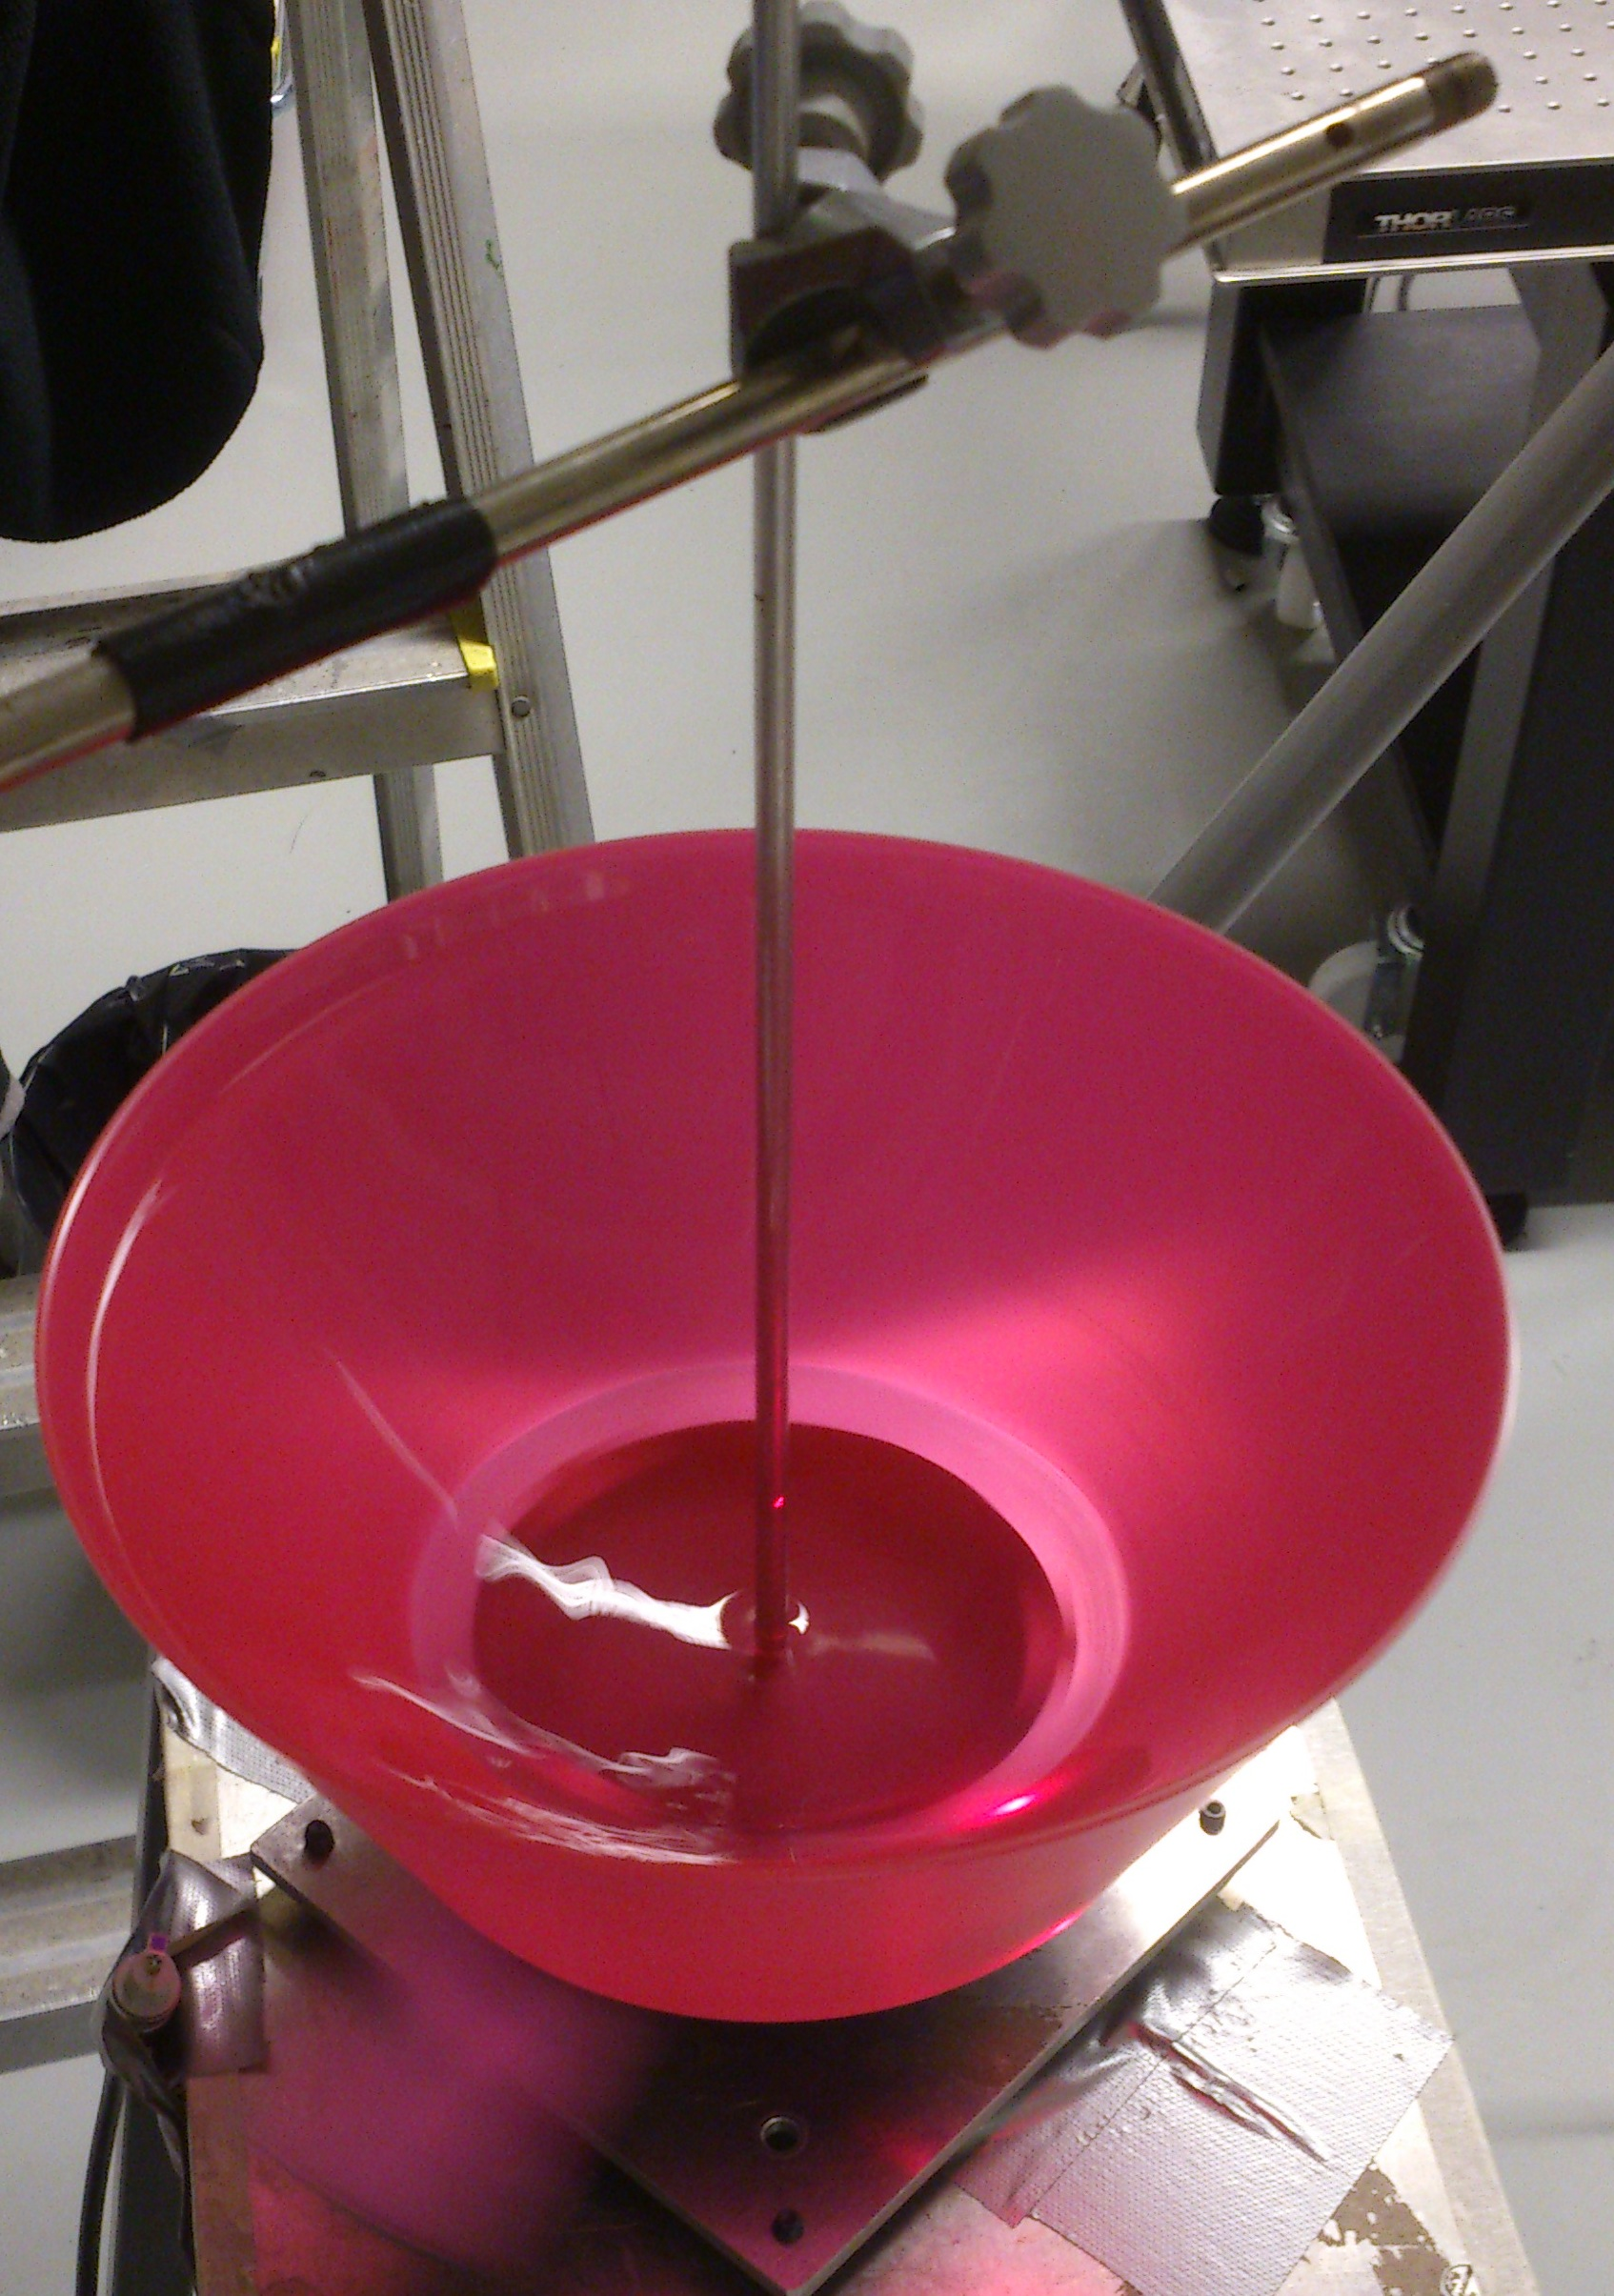
\includegraphics[width=\linewidth]{rot_bowl_pic.jpg}
\resizebox{0.8\linewidth}{!}{\input{rot_bowl_pic.pdf_t}}
\caption{\label{fig:rot_bowl_pic} A photograph of the setup running. The
  reflected beam from a laser pointer (outside frame) can be seen on
  the central rod. } 
\end{figure}

\begin{figure*}\centering
\resizebox{.6\linewidth}{!}{\input{rot_bowl.pdf_t}}
\caption{\label{fig:rot_bowl} Schematic drawing of the setup in
  \figref{fig:rot_bowl_pic} together with the definitions of some of
  the notation used in the calculations. Due to the focal height
  beeing measured slightly outside the exact center of the rod, by
  $\rho$, a small correction $\delta$ has to be made to the measured
  focal height. }
\end{figure*}

\subsection{Calibration}
Firstly the laser pointer has to be perfecly vertical. This can neatly be
calibrated by shining the laser down on the watersurface when it's not
rotating. The laserbeam will then be perfectly vertical when the
reflection hits the source due to the watersurface beeing perfectly
horisontal when still.



\subsection{Corrections}
As shown in \figref{fig:rot_bowl} the measured focal height
$\hat{h}$ is slightly of from the real focal height by 
\begin{equation*}%\label{eq:correction}
\delta=\rho\cot 2\alpha
\end{equation*}
due to a finite width $\rho$ of the central rod. This width is easily
measured with a pair of calipers.

We now have to determine $\alpha$. First of we note that
\begin{equation}\label{eq:dz/dr}
\tan\alpha=\frac{\rd z}{\rd r}=\frac{2 z(r)}{r}.
\end{equation}
Then we see from \figref{fig:rot_bowl} that 
\begin{equation*}
\cot 2\alpha =\frac{\hat{h} - z(r)}{\hat{r}} 
= \frac{\hat{h}}{\hat{r}}-\frac{r}{2\hat{r}}\tan\alpha,
\end{equation*}
where we used \eqref{eq:dz/dr} to substitute $z(r)$ in terms of
$\tan\alpha$. By rewriting the last equation we get
\begin{equation*}
\cot 2\alpha 
-\frac{\hat{h}}{\hat{r}}
+\frac{\hat{r}+\rho}{2\hat{r}}\tan\alpha  = 0.
\end{equation*}
only consisting of known or measured quantities and $\alpha$. From
this stage $\alpha$ can easily be obtained to a satisfying degree with
regular numerical equation solvers.

\section{Results}
The results from the measurements together with the least square fitt
are shown in \figref{fig:data}. The calculated value of the
acceleration of gravity comes out as
\begin{equation*}
g=\unit[9.78\pm 0.13]{m/s^2}
\end{equation*}
the uncertainty given is the standard deviation in the mean.


\begin{figure*}\centering 
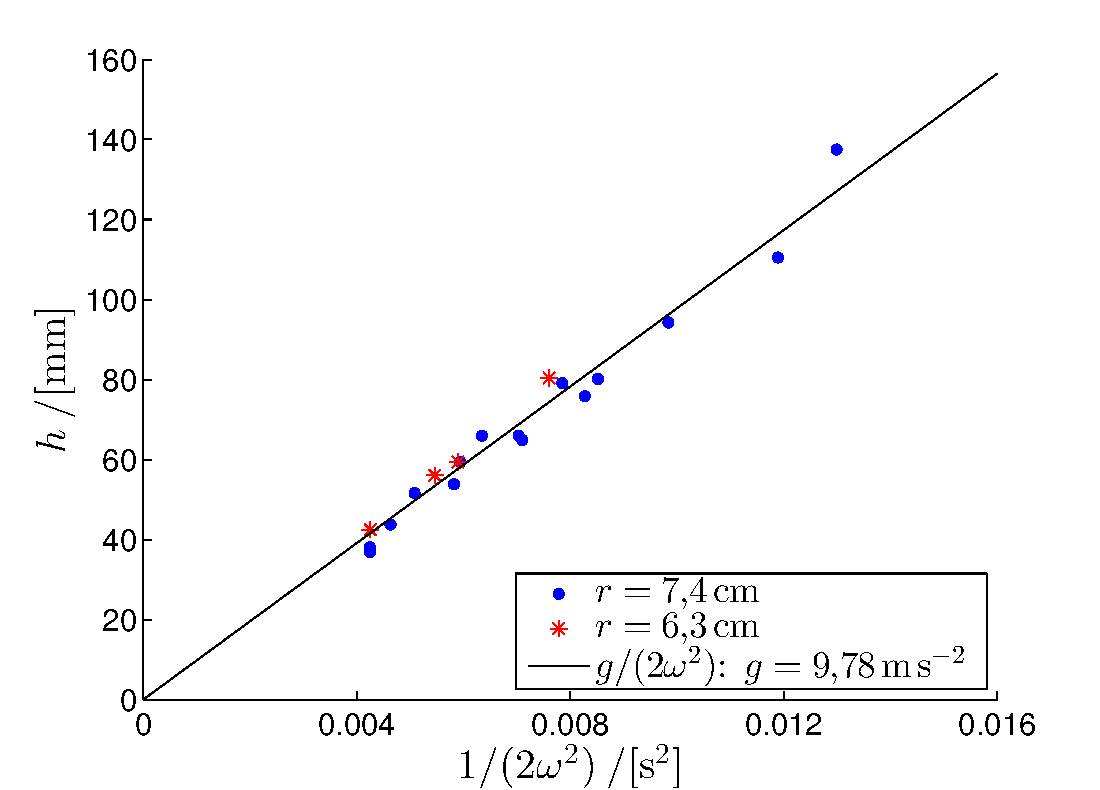
\includegraphics[width=.6\linewidth]{g_minsta_kvadrat.pdf}
\caption{\label{fig:data} Measurements of the focal height $h$ (with
  corrections for a center rod of non-zero width) plotted against
  $1/(2\omega^2)$. The acceleration of gravity $g$ is now given as the
  slope of the least square fitt to these data points. Measurements
  were taken at two different radial distances from the center,
  denoted $r$ in \figref{fig:rot_bowl}.
}
\end{figure*}


\section{Discussion}
As we can see the result comes out close to the familiar value of $g$
as $\unit[9.8]{m/s^2}$. However the error in this method doesn't make
this the most accurate way to measure $g$, bus as stated before this
method is more of an educational experiment than a precision
measurement. And as such this experiment manages to combine both
knowlege in mechanics and optics together with some careful thought
needet to for example find the correction $\delta$.


The significance of the correction due to finite width of the central
rod$\delta$ is quite notable. The value of $g$ comes out to be only
about $\unit[9.2]{m/s^2}$ \emph{without} these corrections. 
%So if a student don't take this into account he or she will notice it
%and have to examine his or her experiment.

Most of the uncertainty in the result arose from small ripples on the
water surface leading to gittery motion of the reflected
laserbeam. Both Berg\cite{Berg1990} and IPhO\cite{IPhO2001} used
glycerin as the liqud in thier experiments which would have lessend
the ripples causing our uncertainties. However as this experiment was
primarily aimed as an experiment with a simple and inexpensive setup
we used water instead. 

The experiment described here can be done as a shorter project in high
school or lab exercise for first year undergraduate students. One
sholud note though that to set up this experiment will around
2--4~hours from scratch to finished measurements depending on the
desired experimental accuracy. If this experiment is done as a project
the student could perhaps also try to compare this method to other
more common methods.


\section*{Acknowledgments}
We are very grateful to the personell in the mashineshop at the
Physics Department at Chalmers. We thank Lars Hellberg and Jan-Åke
Wiman for constructing and balancing the rotating disk so that the
experiments could be performed. 

%%OBS behövs en fil: mybibliography.bib
\bibliographystyle{unsrt}
\bibliography{bibliography}


% \clearpage
% %Gör om sidnumreringen i appendix
% \setcounter{page}{1}
% \renewcommand*{\thepage}{\Alph{section}\arabic{page}}
% %lägger till 'Bilagor' som part för att inte få med någon sidnumrering.
% \addcontentsline{toc}{part}{Bilagor}
% \appendix



\end{document}




